\newcommand*{\nluft}[0]{n_{\text{Luft}}}

\section{Teilversuch 2: Bestimmung des Brechungsindex von Luft}
	Aus der Anleitung ist der Brechungsindex von Luft gegeben durch:
	\begin{equation}
		\nluft = \frac{\lambda P_0}{s}\cdot g + 1 
	\end{equation}
	mit dem entsprechen Fehler:
	\begin{align}
		\Delta \nluft = \nluft \relquad{\lambda,P_0,s,g}
	\end{align}
	wobei $g$ die Steigung des Graphs von $\Delta m$ (die Anzahl der Durchgänge) gegen $P$ (Druck) ist. 

	Wir plotten zunächst die Messwerten und führe mittels \gnuplot{} eine Kurveanpassung der Form $\Delta m = gP + c$ durch (Siehe Appendix \ref{appdx:gnuplottv2}). Ein Messfehler von $\Delta P_i = \SI{1}{\hecto\pascal}$ wird bei der Kurvenanpassung wegen der höhe Anzahl von Messwerten nicht berücksichtigt. 
	\begin{figure}[H]
		\centering
		% GNUPLOT: LaTeX picture with Postscript
\begingroup
  \makeatletter
  \providecommand\color[2][]{%
    \GenericError{(gnuplot) \space\space\space\@spaces}{%
      Package color not loaded in conjunction with
      terminal option `colourtext'%
    }{See the gnuplot documentation for explanation.%
    }{Either use 'blacktext' in gnuplot or load the package
      color.sty in LaTeX.}%
    \renewcommand\color[2][]{}%
  }%
  \providecommand\includegraphics[2][]{%
    \GenericError{(gnuplot) \space\space\space\@spaces}{%
      Package graphicx or graphics not loaded%
    }{See the gnuplot documentation for explanation.%
    }{The gnuplot epslatex terminal needs graphicx.sty or graphics.sty.}%
    \renewcommand\includegraphics[2][]{}%
  }%
  \providecommand\rotatebox[2]{#2}%
  \@ifundefined{ifGPcolor}{%
    \newif\ifGPcolor
    \GPcolortrue
  }{}%
  \@ifundefined{ifGPblacktext}{%
    \newif\ifGPblacktext
    \GPblacktexttrue
  }{}%
  % define a \g@addto@macro without @ in the name:
  \let\gplgaddtomacro\g@addto@macro
  % define empty templates for all commands taking text:
  \gdef\gplbacktext{}%
  \gdef\gplfronttext{}%
  \makeatother
  \ifGPblacktext
    % no textcolor at all
    \def\colorrgb#1{}%
    \def\colorgray#1{}%
  \else
    % gray or color?
    \ifGPcolor
      \def\colorrgb#1{\color[rgb]{#1}}%
      \def\colorgray#1{\color[gray]{#1}}%
      \expandafter\def\csname LTw\endcsname{\color{white}}%
      \expandafter\def\csname LTb\endcsname{\color{black}}%
      \expandafter\def\csname LTa\endcsname{\color{black}}%
      \expandafter\def\csname LT0\endcsname{\color[rgb]{1,0,0}}%
      \expandafter\def\csname LT1\endcsname{\color[rgb]{0,1,0}}%
      \expandafter\def\csname LT2\endcsname{\color[rgb]{0,0,1}}%
      \expandafter\def\csname LT3\endcsname{\color[rgb]{1,0,1}}%
      \expandafter\def\csname LT4\endcsname{\color[rgb]{0,1,1}}%
      \expandafter\def\csname LT5\endcsname{\color[rgb]{1,1,0}}%
      \expandafter\def\csname LT6\endcsname{\color[rgb]{0,0,0}}%
      \expandafter\def\csname LT7\endcsname{\color[rgb]{1,0.3,0}}%
      \expandafter\def\csname LT8\endcsname{\color[rgb]{0.5,0.5,0.5}}%
    \else
      % gray
      \def\colorrgb#1{\color{black}}%
      \def\colorgray#1{\color[gray]{#1}}%
      \expandafter\def\csname LTw\endcsname{\color{white}}%
      \expandafter\def\csname LTb\endcsname{\color{black}}%
      \expandafter\def\csname LTa\endcsname{\color{black}}%
      \expandafter\def\csname LT0\endcsname{\color{black}}%
      \expandafter\def\csname LT1\endcsname{\color{black}}%
      \expandafter\def\csname LT2\endcsname{\color{black}}%
      \expandafter\def\csname LT3\endcsname{\color{black}}%
      \expandafter\def\csname LT4\endcsname{\color{black}}%
      \expandafter\def\csname LT5\endcsname{\color{black}}%
      \expandafter\def\csname LT6\endcsname{\color{black}}%
      \expandafter\def\csname LT7\endcsname{\color{black}}%
      \expandafter\def\csname LT8\endcsname{\color{black}}%
    \fi
  \fi
    \setlength{\unitlength}{0.0500bp}%
    \ifx\gptboxheight\undefined%
      \newlength{\gptboxheight}%
      \newlength{\gptboxwidth}%
      \newsavebox{\gptboxtext}%
    \fi%
    \setlength{\fboxrule}{0.5pt}%
    \setlength{\fboxsep}{1pt}%
\begin{picture}(8640.00,5760.00)%
    \gplgaddtomacro\gplbacktext{%
      \csname LTb\endcsname%%
      \put(682,704){\makebox(0,0)[r]{\strut{}$-5$}}%
      \put(682,1253){\makebox(0,0)[r]{\strut{}$0$}}%
      \put(682,1803){\makebox(0,0)[r]{\strut{}$5$}}%
      \put(682,2352){\makebox(0,0)[r]{\strut{}$10$}}%
      \put(682,2902){\makebox(0,0)[r]{\strut{}$15$}}%
      \put(682,3451){\makebox(0,0)[r]{\strut{}$20$}}%
      \put(682,4000){\makebox(0,0)[r]{\strut{}$25$}}%
      \put(682,4550){\makebox(0,0)[r]{\strut{}$30$}}%
      \put(682,5099){\makebox(0,0)[r]{\strut{}$35$}}%
      \put(814,484){\makebox(0,0){\strut{}$450$}}%
      \put(2052,484){\makebox(0,0){\strut{}$500$}}%
      \put(3290,484){\makebox(0,0){\strut{}$550$}}%
      \put(4529,484){\makebox(0,0){\strut{}$600$}}%
      \put(5767,484){\makebox(0,0){\strut{}$650$}}%
      \put(7005,484){\makebox(0,0){\strut{}$700$}}%
      \put(8243,484){\makebox(0,0){\strut{}$750$}}%
    }%
    \gplgaddtomacro\gplfronttext{%
      \csname LTb\endcsname%%
      \put(209,2901){\rotatebox{-270}{\makebox(0,0){\strut{}Anzahl der Durchgängen $\Delta m$ (Einheitslos)}}}%
      \put(4528,154){\makebox(0,0){\strut{}Druck $P$ ($\si{\hecto\pascal}$)}}%
      \csname LTb\endcsname%%
      \put(7256,1977){\makebox(0,0)[r]{\strut{}Messung 1}}%
      \csname LTb\endcsname%%
      \put(7256,1757){\makebox(0,0)[r]{\strut{}Messung 2}}%
      \csname LTb\endcsname%%
      \put(7256,1537){\makebox(0,0)[r]{\strut{}Messung 3}}%
      \csname LTb\endcsname%%
      \put(7256,1317){\makebox(0,0)[r]{\strut{}$0,12876P + (-63,61708)$}}%
      \csname LTb\endcsname%%
      \put(7256,1097){\makebox(0,0)[r]{\strut{}$0,12976P + (-65,87209)$}}%
      \csname LTb\endcsname%%
      \put(7256,877){\makebox(0,0)[r]{\strut{}$0,15166P + (-73,36752)$}}%
      \csname LTb\endcsname%%
      \put(4528,5429){\makebox(0,0){\strut{}Druck gegen die Anzahl der Durchgängen}}%
    }%
    \gplbacktext
    \put(0,0){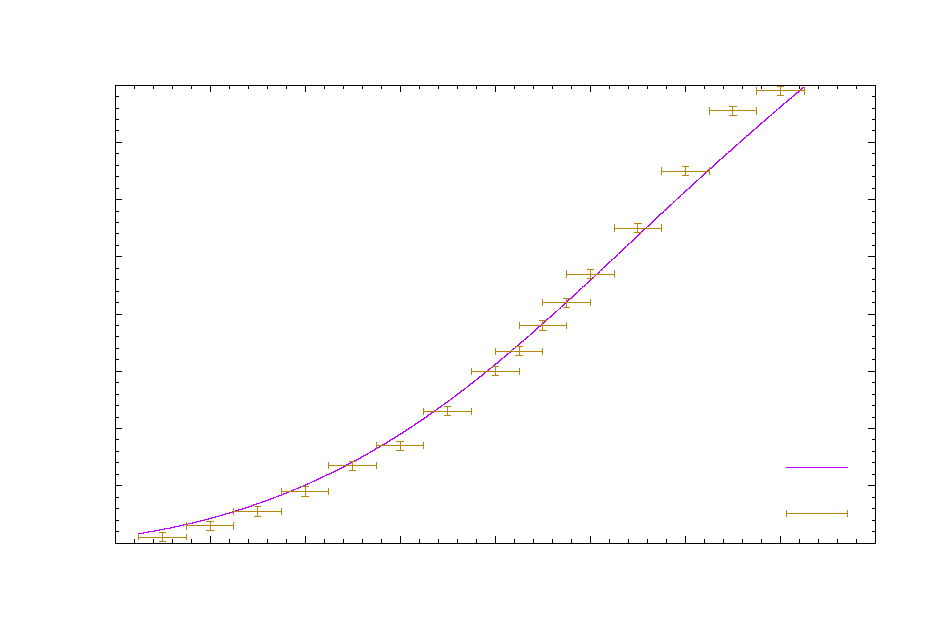
\includegraphics[width={432.00bp},height={288.00bp}]{tv2-plot}}%
    \gplfronttext
  \end{picture}%
\endgroup

		\caption{\centering Druck gegen die Anzahl der Durchgängen}
		\label{fig:tv2-plot}
		\vspace{-1em}
	\end{figure}
	Als Ergebnis erhalten wir:
	\begin{center}
		\begin{tabular}{llll}
			\toprule
			Messung & $g/\si{\per\hecto\pascal}$ & $c$ & $\chi^2_\text{red}$ \\
			\midrule
				$1$ & \num{0,12876(67)} & \num{-63,61708(39587)} & \num{0,01169} \\
				$2$ & \num{0,12976(147)} & \num{-65,87209(89462)} & \num{0,05631} \\
				$3$ & \num{0,15166(586)} & \num{-73,36752(333679)} & \num{0,65034} \\
			\bottomrule
		\end{tabular}
	\end{center}
	Gerundet:
	\begin{center}
		\begin{tabular}{lll}
			\toprule
			Messung & $g/\si{\per\hecto\pascal}$ & $c$ \\
			\midrule
				$1$ & \num{0,1288(7)}  & \num{-63,6(4)}\\
				$2$ & \num{0,1298(15)} & \num{-65,9(9)}\\
				$3$ & \num{0,152(6)}   & \num{-73(4)}\\
			\bottomrule
		\end{tabular}
	\end{center}
	Nun berechnen wir den Mittelwert von $g$. Wir vernachlässigen jegliche Fehler bei der einzelnen $g$-Werten und nehmen die statische Schwankung $$\Delta g = \frac{g_{\text{max}} - g_\text{min}}{2}$$ als der Fehler, da diese Schwankung viel große ist. Es ist in diesem Fall wegen der niedrigen Anzahl von $g$-Werten nicht sinnvoll, die Standardabweichung zu nehmen. 

	Wir erhalten somit $\overline{g} = \SI{0.137(12)}{\per\hecto\pascal}$. Im Folgenden ist $g = \overline{g}$.

	Mit der Messwerten:
	\begin{center}
		\begin{tabular}{lll}
			\toprule
			Variable & Wert & Bedeutung \\
			\midrule
			$\lambda$ & \SI{520(20)}{\nano\meter} & Wellenlänge des Lasers \\
			$P_0$ & \SI{9.51(1)e4}{\pascal} & Atmosphäredruck im Raum \\
			$s$ & \SI{256.38(3)}{\milli\meter} & Optische Länge der Küvette \\
			$g$ & \SI{1.37(12)e-3}{\per\pascal} & Durchschnittliche Steigung \\
			\bottomrule
		\end{tabular}
	\end{center}
	erhalten wir:
	\begin{align}
		\nluft 
		&= \frac{(\SI{520e-9}{\meter})(\SI{9.51e4}{\pascal})}{\SI{256.38e-3}{\meter}}\cdot (\SI{1.37e-3}{\per\pascal}) + 1 \notag \\
		&= \num{1.000264253} \sigfig{10} \\
		\Delta\nluft 
		&= (\num{1.000264253}) \sqrt{
			\left(\frac{20}{520}\right)^2 +
			\left(\frac{0.01}{9.51}\right)^2 +
			\left(\frac{0.03}{256.38}\right)^2 +
			\left(\frac{0.12}{1.37}\right)^2
		} \notag \\
		&= \num{0.10} \sigfig{2}
	\end{align}
	Somit erhalten wir als Endergebnis: $\nluft = \num{1.00(10)}$.

	Dieses Ergebnis stimmt mit der Literaturwert $n_\text{Luft, Lit} = 1.000269$ überein. Der Fehler ist aber sehr groß, was hauptsächlich zur
	\begin{itemize}
		\item Unsicherheit in der Wellenlänge des Lasers und
		\item Unsicherheit bei dem selbstständigen Zählen der Durchgängen
	\end{itemize}
	zurückzuführen ist. 